\section{Findings}

\subsection{Technical evaluation of the proposal suitability}

The aim of the proposal is to detect and report communications in which CSAM is present. In particular, the types of CSAM to be recognised are known CSAM, unknown CSAM, and child sexual solicitation (grooming).

While the proposal does not focus on the implementation details, the impact assessment accompanying the proposition presents two technical annexes. Annex 8 explains technologies covered in section \ref{ss:det_algo}. Annex 9 evaluates different approaches for CSS and SSS, introduced in section \ref{ss:scanning}.

\subsubsection{Detection of known CSAM}

To detect previosuly known CSAM in an E2EE communication, it is proposed in Annex 9 to use server side scanning implementing a system similar to Microsoft's PhotoDNA but hashing the shared content on client-side before the encryption that happens before the material is sent\cite{eu2022impact}. 

While it is stated in Annex 9, the proposal fails to recognise that perception hashing does not perform well in an adversarial context. 

To elaborate on this, it is possible to generate images that will trigger false positives by injecting adversarial noise in a non-CSAM image to make hashing algorithm an hash that will collide with CSAM hash\footnote{Such an attack can be performed against Apple's Neuralhash as shown in \url{https://github.com/greentfrapp/apple-neuralhash-attack}}.

To avoid these types of attacks, the assessment aims at following a "security by obscurity" desing to avoid leacking of the algorithm. This type of design is not state of the art and is not secure by design by itself\cite{SandO}. Furthermore, the algorithm will have to be run on client side, making maintaining the secrecy of the hasher implementation difficult\footnote{See \url{https://github.com/AsuharietYgvar/AppleNeuralHash2ONNX}}.

\subsubsection{Detection of unknown CSAM}

As previosuly described, to detect unknown CSAM machine learning classifiers are needed. Discussing the context in which the communication is E2E encrypted, the impact assessment propose the deployment of the classifier model on client side and operating the classification previosly the encryption of the media. Furthermore, this approach is difficult to implement especially on smartphones and other devices with lower computational capabilities. 

Morevoer, both the accompanying and the complementary impact assessment report that there exist a classifier for detecting new CSAM, Thorn's Safer, with a precision of 99.9\% and a recall of 80\%\cite{eu2022impact} \cite{eu2023impact}. Unfortunately, no proof is provided to support such claims and the citation linking to the benchmarking platform redirect to a benchmarking platform for perceptual hashing algorithms and not for classifiers of previously unknown CSAM\footnote{The link to the benchmarking platform is \url(https://perception.thorn.engineering/en/latest/examples/benchmarking.html)}.

Furthermore, the performance reported in these documents are optimistic at least if compared with what has been summarize in section \ref{sss:ML}, and also taking into consideration that the Thorn's model for CSAM detection is deployed on server side\cite{Thorn} having access to higher computing power.

\subsubsection{Sexual solicitation of children}

Also in this case, ML classifiers are required to scan conversations and flag grooming behaviour. Again, in E2EE communications the model must be deployed client-side. Text-based classifiers are easier to implement client-side than models based on other media as also noted in Annex 9 of the complementary impact assessment\cite{eu2022impact}. Furthemore, server-side based solutions developed under project Arthemis are reported to have an accuracy of only 88\%\cite{eu2022impact}.

\subsubsection{Avoiding detection during CSAM sharing}

A simple way to avoid detection under this proposed solution is to encrypt the media before sharing on the controlled platform. This issue is also been noted in the EDPB-EDPS Joint Opinion\cite{Joint} but nevera adressed in any other reviewed document.

To elaborate on this, two adversaries that aim at maintaining the file sharing anonymous could engage in a key exchange as in an insecure communication channel. Having computed a shared secret, such secret is used to compute a symmetric key used to encrypt the media.

The following bash code and figure show how two users can share media without the system being able to detect CSAM material.
\\
\begin{minipage}{0.5\textwidth}

    \lstset{
        language=bash,
        basicstyle=\ttfamily\tiny,
        keywordstyle=\color{blue},
        commentstyle=\color{green!50!black},
        stringstyle=\color{orange},
        showstringspaces=false,
        breaklines=true,
        frame=single,
        backgroundcolor=\color{gray!10},
        captionpos=b,
    }

    \begin{lstlisting}
# Generate EC parameters for the prime256v1 (secp256v1) curve and save them to ecparam.pem
openssl ecparam -name prime256v1 -out ecparam.pem
# Generate a private key for Party 1 using the prime256v1 curve and save it to party1_private_key.pem
openssl ecparam -name prime256v1 -genkey -noout -out party1_private_key.pem
# Extract and save the public key from Party 1's private key to party1_public_key.pem
openssl ec -in party1_private_key.pem -pubout -out party1_public_key.pem
# Derive a shared secret using Party 1's private key and Party 2's public key, saving the result to shared_secret.bin
openssl pkeyutl -derive -inkey party1_private_key.pem  -peerkey party2_public_key.pem -out shared_secret.bin
# Encrypt body.bin using AES-256-CBC with the shared secret (no salt used) and save the output to body.ecb.bin
openssl enc -aes-256-cbc -nosalt -pass file:./shared_secret.bin -in body.bin -out body.ecb.bin
    \end{lstlisting}
    \captionof{lstlisting}{Client 1 exchange a secret over unsecure channel and image encryption}
\end{minipage}%
\hfill
\begin{minipage}{0.4\textwidth}
    \centering
    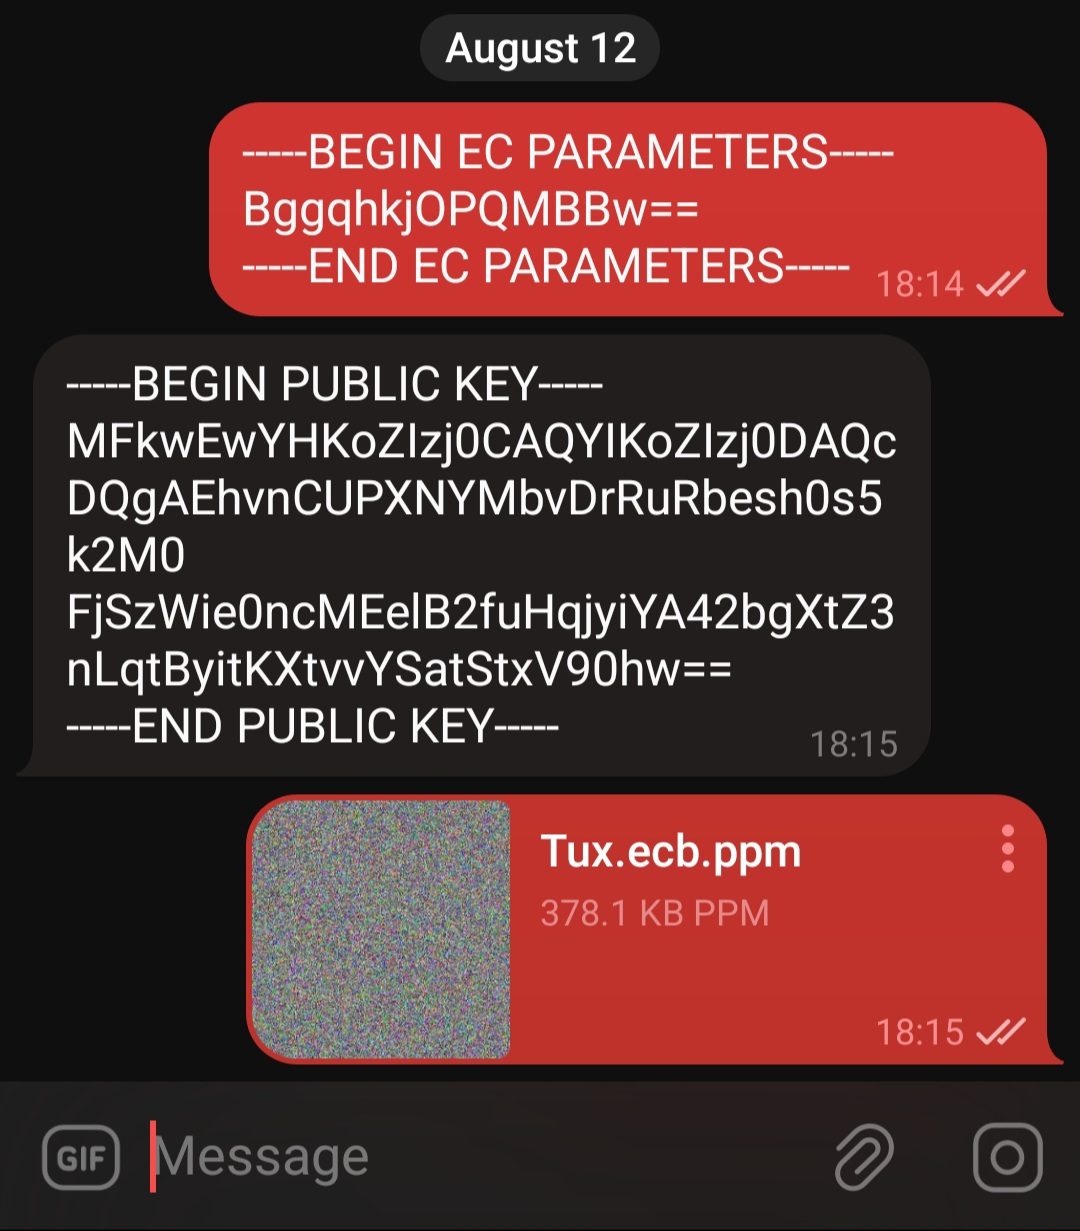
\includegraphics[keepaspectratio,width=0.85\textwidth]{05-results/img/enc_chat.jpg}
    \captionof{figure}{ECDH key exchange and AES encrypted image sharing}
\end{minipage}

\subsection{Relevant ECHR Cases}

Following three cases discussed by the European Court of Human Rights about mass surveillance are presented. All three cases present discussions relating to violations in Articles 8 and 10 of the EU Charter of Fundamental Rights.

\subsubsection{Big Brother et al. v. the United Kingdom}

As described in \cite{big_brother}, following the publication of the Snowden files that revealed the existence of an international surveillance system, the applicants complained an interference with their rights expressed by Article 8 and Article 10. The applicants claimed that their communications or communication data were tracked by the UK intelligence or obtained via service providers and/or via foreign intelligence.

The court ruled that there was indeed an interference with both Article 8 and Article 10 since the bulk intercpetion was taking place in secret. In particular, the Court defined bulk interception as a four stage process in which (a) there is the interception and initial retention of communication data, (b) application of specific selectors to the retained data, e.g. queries, (c) examination of the selected data by analysts, (d) data retention. 

Subsequently, the Court stated that, in a lawful bulk interception, the State should present clearly the grounds upon which the interception may take place.


